\documentclass[conference]{IEEEtran}

\usepackage{amsmath,amssymb}
\usepackage{graphicx}
\usepackage{booktabs}
\usepackage{array}
\usepackage{multirow}
\usepackage{cite}
\usepackage{url}
\usepackage{microtype}
\usepackage[hidelinks]{hyperref}
\hypersetup{pdftitle={Cancer Classification Using Probabilistic Machine Learning},pdfauthor={Ojas Kumar Kashyap; Iraban Bhattacharya}}

\graphicspath{{figures/}}
\interdisplaylinepenalty=2500

\title{Cancer Classification Using Probabilistic Machine Learning: A Bayesian Approach with Gaussian Naive Bayes}

\author{\IEEEauthorblockN{Ojas Kumar Kashyap and Iraban Bhattacharya}
\IEEEauthorblockA{School of Computer Science and Engineering, Vellore Institute of Technology, Vellore, India\\
Probability and Statistics (BAMAT207), Track 6: AI, Machine Learning and Probability\\
}}

\begin{document}
\maketitle

\begin{abstract}
This project applies probability and statistical estimation to two related but distinct classification problems. The primary experiment predicts benign or malignant breast tumours using the Breast Cancer Wisconsin (Diagnostic) dataset, which contains 569 records described by 30 numeric cell-nucleus measurements. A secondary experiment studies the recorded biopsy outcome in the UCI Cervical Cancer (Risk Factors) dataset. The datasets are analysed separately because their features and target labels have different meanings. Gaussian Naive Bayes (GNB) is implemented from scratch using class priors, maximum-likelihood estimates of Gaussian means and variances, conditional likelihoods, and Bayes' theorem. Its predictions are checked against the scikit-learn implementation. Logistic Regression, class-balanced Logistic Regression, and a prior baseline are used for comparison. With a stratified 80:20 split and fixed random seed, scratch GNB achieves 93.86\% accuracy, 83.33\% malignant-class recall, and 0.993 ROC-AUC on the breast test set. Balanced Logistic Regression achieves the highest breast test-set accuracy, balanced accuracy, recall, and F1 among the tested models, while standard Logistic Regression has the highest breast ROC-AUC and average precision. Results differ substantially for the cervical task: GNB detects 10 of 11 positive test biopsy outcomes but produces 148 false positives, giving only 6.33\% precision and 10.78\% accuracy. Five-fold cross-validation on training data is also reported. The experiments demonstrate Bayes' theorem, conditional probability, Gaussian modelling, likelihood estimation, and the importance of class-sensitive evaluation. These results are educational experiments on public datasets and do not establish clinical validity.
\end{abstract}

\begin{IEEEkeywords}
Bayesian inference, Gaussian Naive Bayes, cancer-related classification, conditional probability, Gaussian distribution, likelihood estimation, imbalanced classification, Logistic Regression.
\end{IEEEkeywords}

\section{Introduction}
Classification is a common machine-learning task in which a model assigns an observation to one of a set of categories using measured attributes. In a health-related setting, measurements may describe cell morphology, demographic characteristics, habits, or medical history. These variables provide a practical context for studying the relation between probability theory and data-driven classification. The focus of this project is not to develop a clinical product, but to implement a probabilistic model, inspect how its predictions are formed, and evaluate the consequences of modelling assumptions.

The primary experiment uses the Breast Cancer Wisconsin (Diagnostic) dataset. Its 30 continuous predictors are derived from digitised fine-needle-aspirate images and describe characteristics of cell nuclei, including radius, texture, perimeter, area, smoothness, compactness, concavity, symmetry, and fractal dimension \,\cite{uciBreast,street}. Ten underlying measurements are represented in mean, standard-error, and worst-value forms. The recorded diagnosis is either benign or malignant.

An extension applies the same overall experimental workflow to the UCI Cervical Cancer (Risk Factors) dataset. This dataset includes demographic information, habits, and historical medical records, with missing values reported for several variables \cite{uciCervical,fernandes}. Here, the chosen target is the recorded \texttt{Biopsy} result. It is deliberately not described as a general cervical-cancer diagnosis: a biopsy outcome is a specific label in this dataset, and the experiment does not establish a screening or diagnostic system.

Both experiments use Gaussian Naive Bayes as the principal probability model. A from-scratch implementation makes the calculations inspectable and is validated against scikit-learn's implementation. Logistic Regression and a class-balanced variant provide comparison points. Metrics include accuracy, balanced accuracy, precision, recall, F1-score, ROC-AUC, and average precision (area under the precision-recall curve). The second dataset is especially useful for demonstrating why accuracy can be misleading when the positive class is rare.

\section{Problem Statement and Objectives}
The central problem is to estimate the probability of a class label given an input feature vector and to assign the most probable class. For the breast dataset, the classes are benign (0) and malignant (1). For the cervical dataset, the classes are biopsy-negative (0) and biopsy-positive (1). Separate models are fitted for the two tasks; records and features are not combined.

The objectives are: (1) estimate class prior probabilities from training data; (2) estimate feature-wise Gaussian parameters; (3) calculate likelihoods and posterior probabilities using Bayes' theorem; (4) implement Gaussian Naive Bayes from scratch and numerically validate it against a library implementation; (5) compare models on held-out test data and by stratified five-fold cross-validation within the training partition; and (6) interpret errors, class imbalance, and model assumptions without making clinical claims.

\section{Related Work and Background}
\subsection{Dataset context}
Street, Wolberg, and Mangasarian described extraction of nuclear features from digitised fine-needle-aspirate images for breast tumour diagnosis \cite{street}. The UCI Breast Cancer Wisconsin (Diagnostic) collection provides 569 observations and 30 continuous input features \cite{uciBreast}. Its well-defined numeric feature set makes it appropriate for demonstrating class-conditional density estimation. However, several morphological measurements are strongly correlated, which is relevant to the independence assumption made by Naive Bayes.

The UCI Cervical Cancer (Risk Factors) dataset contains 858 original records and 36 listed features/target attributes; the repository notes that some answers are missing \cite{uciCervical}. Related work by Fernandes \textit{et al.} explores transfer learning with partially observed information for cervical-cancer screening problems \cite{fernandes}. The present experiment is narrower: it uses risk-factor/history inputs to estimate the recorded \texttt{Biopsy} outcome, excludes other diagnosis/screening outcomes from the predictors, and evaluates a small set of standard classifiers. Consequently, results should not be compared directly with studies that use different targets, modalities, data partitions, or preprocessing procedures.

\subsection{Probabilistic classification}
Naive Bayes classifiers apply Bayes' theorem and simplify the class-conditional likelihood by assuming that features are conditionally independent given the class. Gaussian Naive Bayes uses a Gaussian density for each feature within each class \cite{bishop,sklearnNB}. This combination is computationally simple and allows the contribution of priors and class-specific feature distributions to be discussed explicitly. Its independence assumption is restrictive when predictors are correlated; the Gaussian assumption is also only an approximation for binary and discrete risk-factor inputs.

Logistic Regression provides a discriminative comparison model. Its class probability is estimated directly from a linear function of the predictors rather than by multiplying class-conditional Gaussian densities. A class-balanced Logistic Regression model changes the training penalty so that errors on the less frequent class receive more weight. For highly imbalanced binary data, precision-recall analysis can be informative alongside ROC analysis because it explicitly tracks positive-class precision and recall \cite{saito}.

\section{Datasets and Preprocessing}
\subsection{Breast Cancer Wisconsin (Diagnostic)}
The downloaded CSV initially contains 569 rows, an identifier, a diagnosis label, 30 numeric features, and an entirely empty extra column. The identifier and empty column are removed. Diagnosis is mapped to benign = 0 and malignant = 1; all 569 observations are retained, with no duplicate rows or missing values in the model inputs found in the notebook's inspection. The class counts are 357 benign (62.74\%) and 212 malignant (37.26\%). The final modelling matrix contains 30 input features.

The split is stratified, with 455 observations for training and 114 for testing. The training class counts are 285 benign and 170 malignant, producing estimated priors $P(B)=0.626374$ and $P(M)=0.373626$. The test set contains 72 benign and 42 malignant samples. No feature is dropped by the training-only missingness or constant-column rules.

\subsection{Cervical Cancer (Risk Factors)}
The original data contain 858 records. String values such as \texttt{?} are converted to missing numeric values. Twenty-three exact duplicate rows are removed, leaving 835 records: 781 biopsy-negative and 54 biopsy-positive (6.47\% positive). The target is \texttt{Biopsy}. Other diagnosis or screening columns (\texttt{Dx:Cancer}, \texttt{Dx:CIN}, \texttt{Dx:HPV}, \texttt{Dx}, \texttt{Hinselmann}, \texttt{Schiller}, and \texttt{Citology}) are excluded from the feature matrix to reduce target leakage. This leaves 28 candidate risk-factor/history predictors before training-only filtering.

A stratified split gives 668 training records (625 negative, 43 positive) and 167 test records (156 negative, 11 positive). The training-set priors are $P(\text{negative})=0.935629$ and $P(\text{positive})=0.064371$. Within training data, two predictor columns exceeding 50\% missingness and two constant columns are removed, leaving 24 features. Median imputation is fitted on the training data and then applied to the held-out test data. This avoids computing imputation values from test observations.

\begin{table*}[!t]
\centering
\caption{Summary of the Two Separate Experiments}
\label{tab:data}
\scriptsize
\setlength{\tabcolsep}{5pt}
\begin{tabular}{p{2.05cm}rrrrp{2.4cm}rr}
\toprule
Experiment & Original rows & Rows analysed & Candidate inputs & Inputs used & Target classes & Train/test & Positive test cases \\
\midrule
Breast diagnostic & 569 & 569 & 30 & 30 & Benign / malignant & 455 / 114 & 42 malignant \\
Cervical risk factors & 858 & 835 & 28 & 24 & Biopsy-negative / biopsy-positive & 668 / 167 & 11 positive \\
\bottomrule
\end{tabular}
\end{table*}

\subsection{Exploratory data analysis}
Exploratory analysis includes descriptive statistics, class-distribution plots, feature distributions, correlation heatmaps, and class-specific Gaussian density curves. The breast target is moderately imbalanced. Several breast morphometric variables are strongly correlated, as expected for related size and shape measurements. This indicates that the conditional-independence assumption should be regarded as a modelling simplification rather than a literal description of the data.

The cervical target is much more imbalanced. The positive biopsy class represents 54 of 835 records before splitting and only 11 test records. Most risk-factor fields are binary or discrete indicators, and some variables contain substantial missingness. These characteristics make the cervical experiment a useful stress test of the model and its evaluation metrics, but they also make its results less stable and the continuous-Gaussian likelihood assumption less realistic.

\begin{figure*}[!t]
\centering
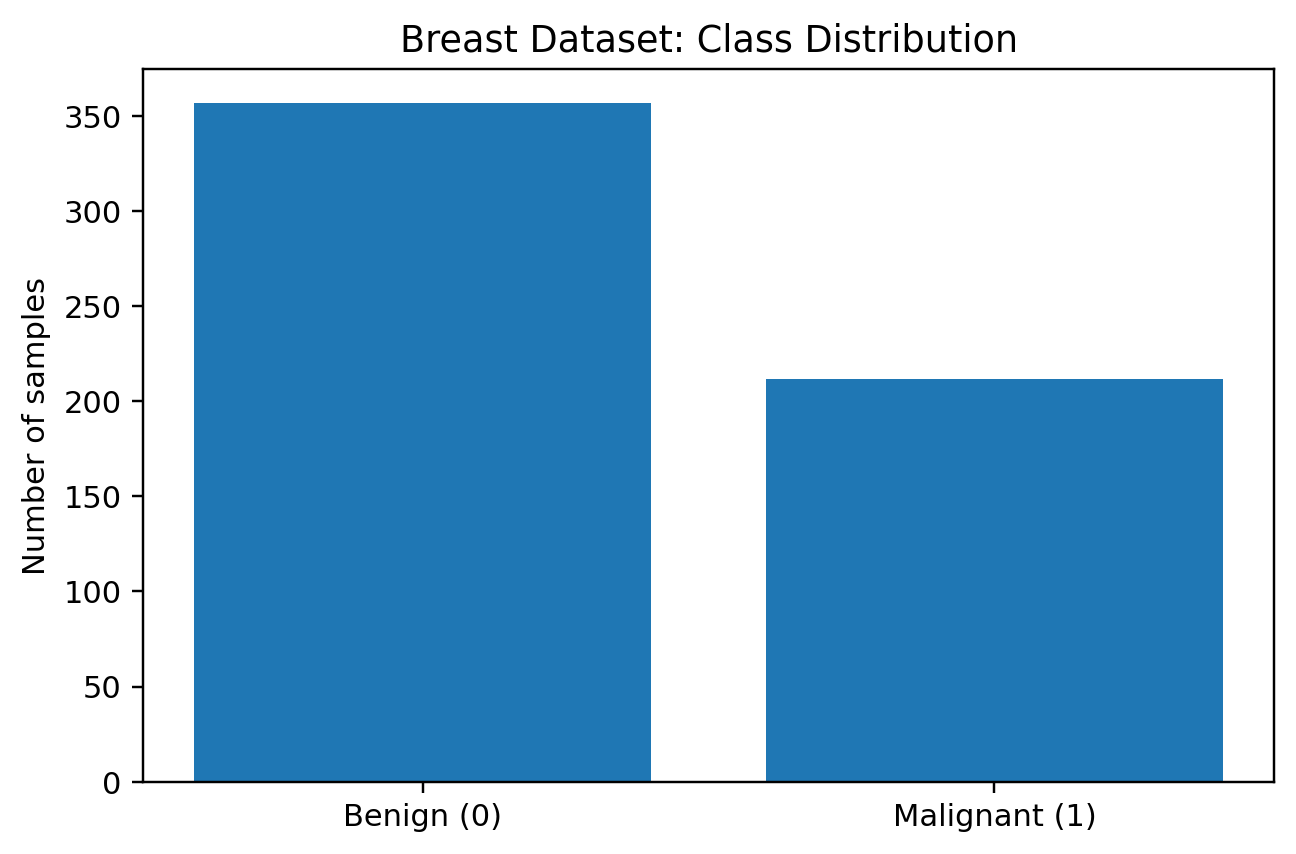
\includegraphics[width=0.47\textwidth]{breast_class_distribution.png}\hfill
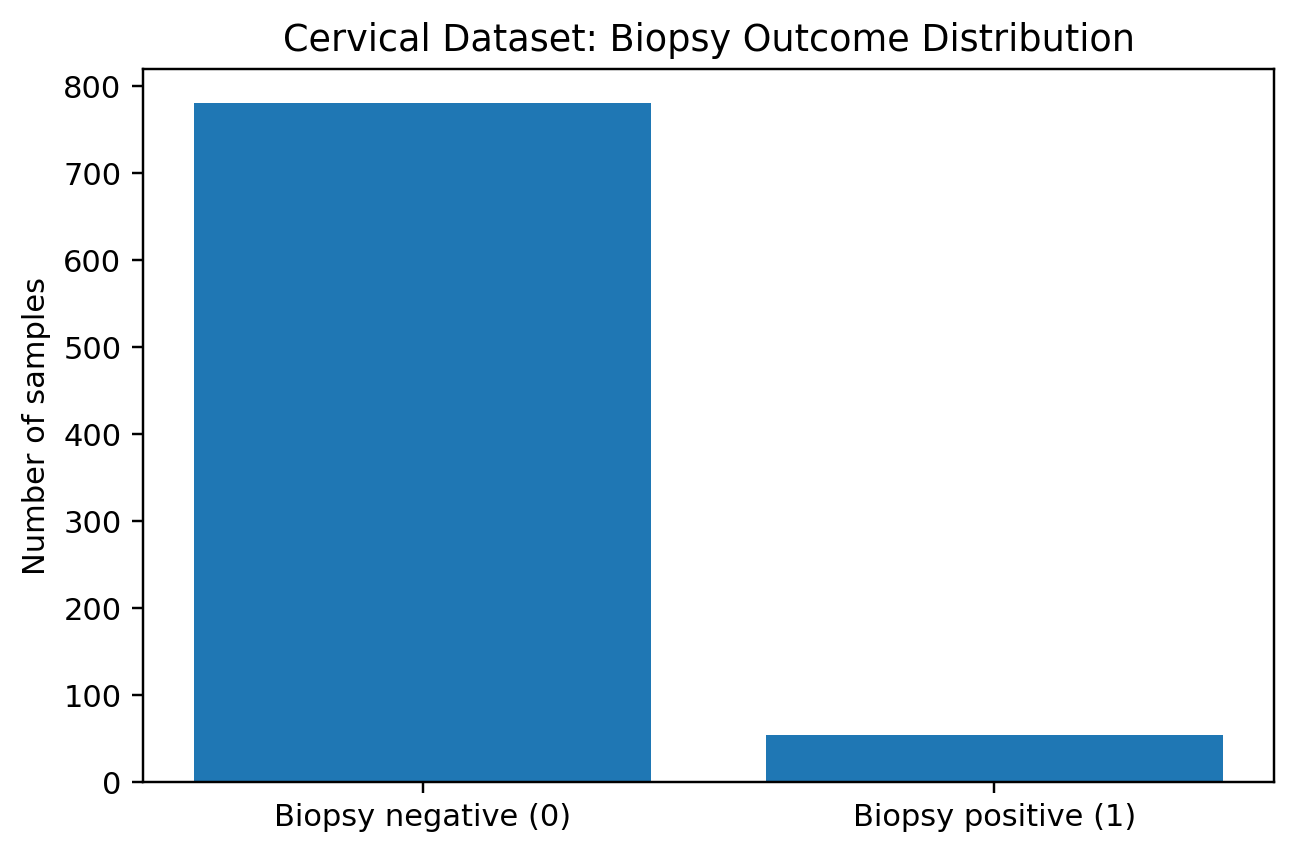
\includegraphics[width=0.47\textwidth]{cervical_biopsy_class_distribution.png}
\caption{Class counts for the separate datasets. Left: 357 benign and 212 malignant breast cases. Right: 781 biopsy-negative and 54 biopsy-positive cervical records after exact-duplicate removal. The axes and class labels refer to different outcomes.}
\label{fig:classes}
\end{figure*}

\begin{figure*}[!t]
\centering
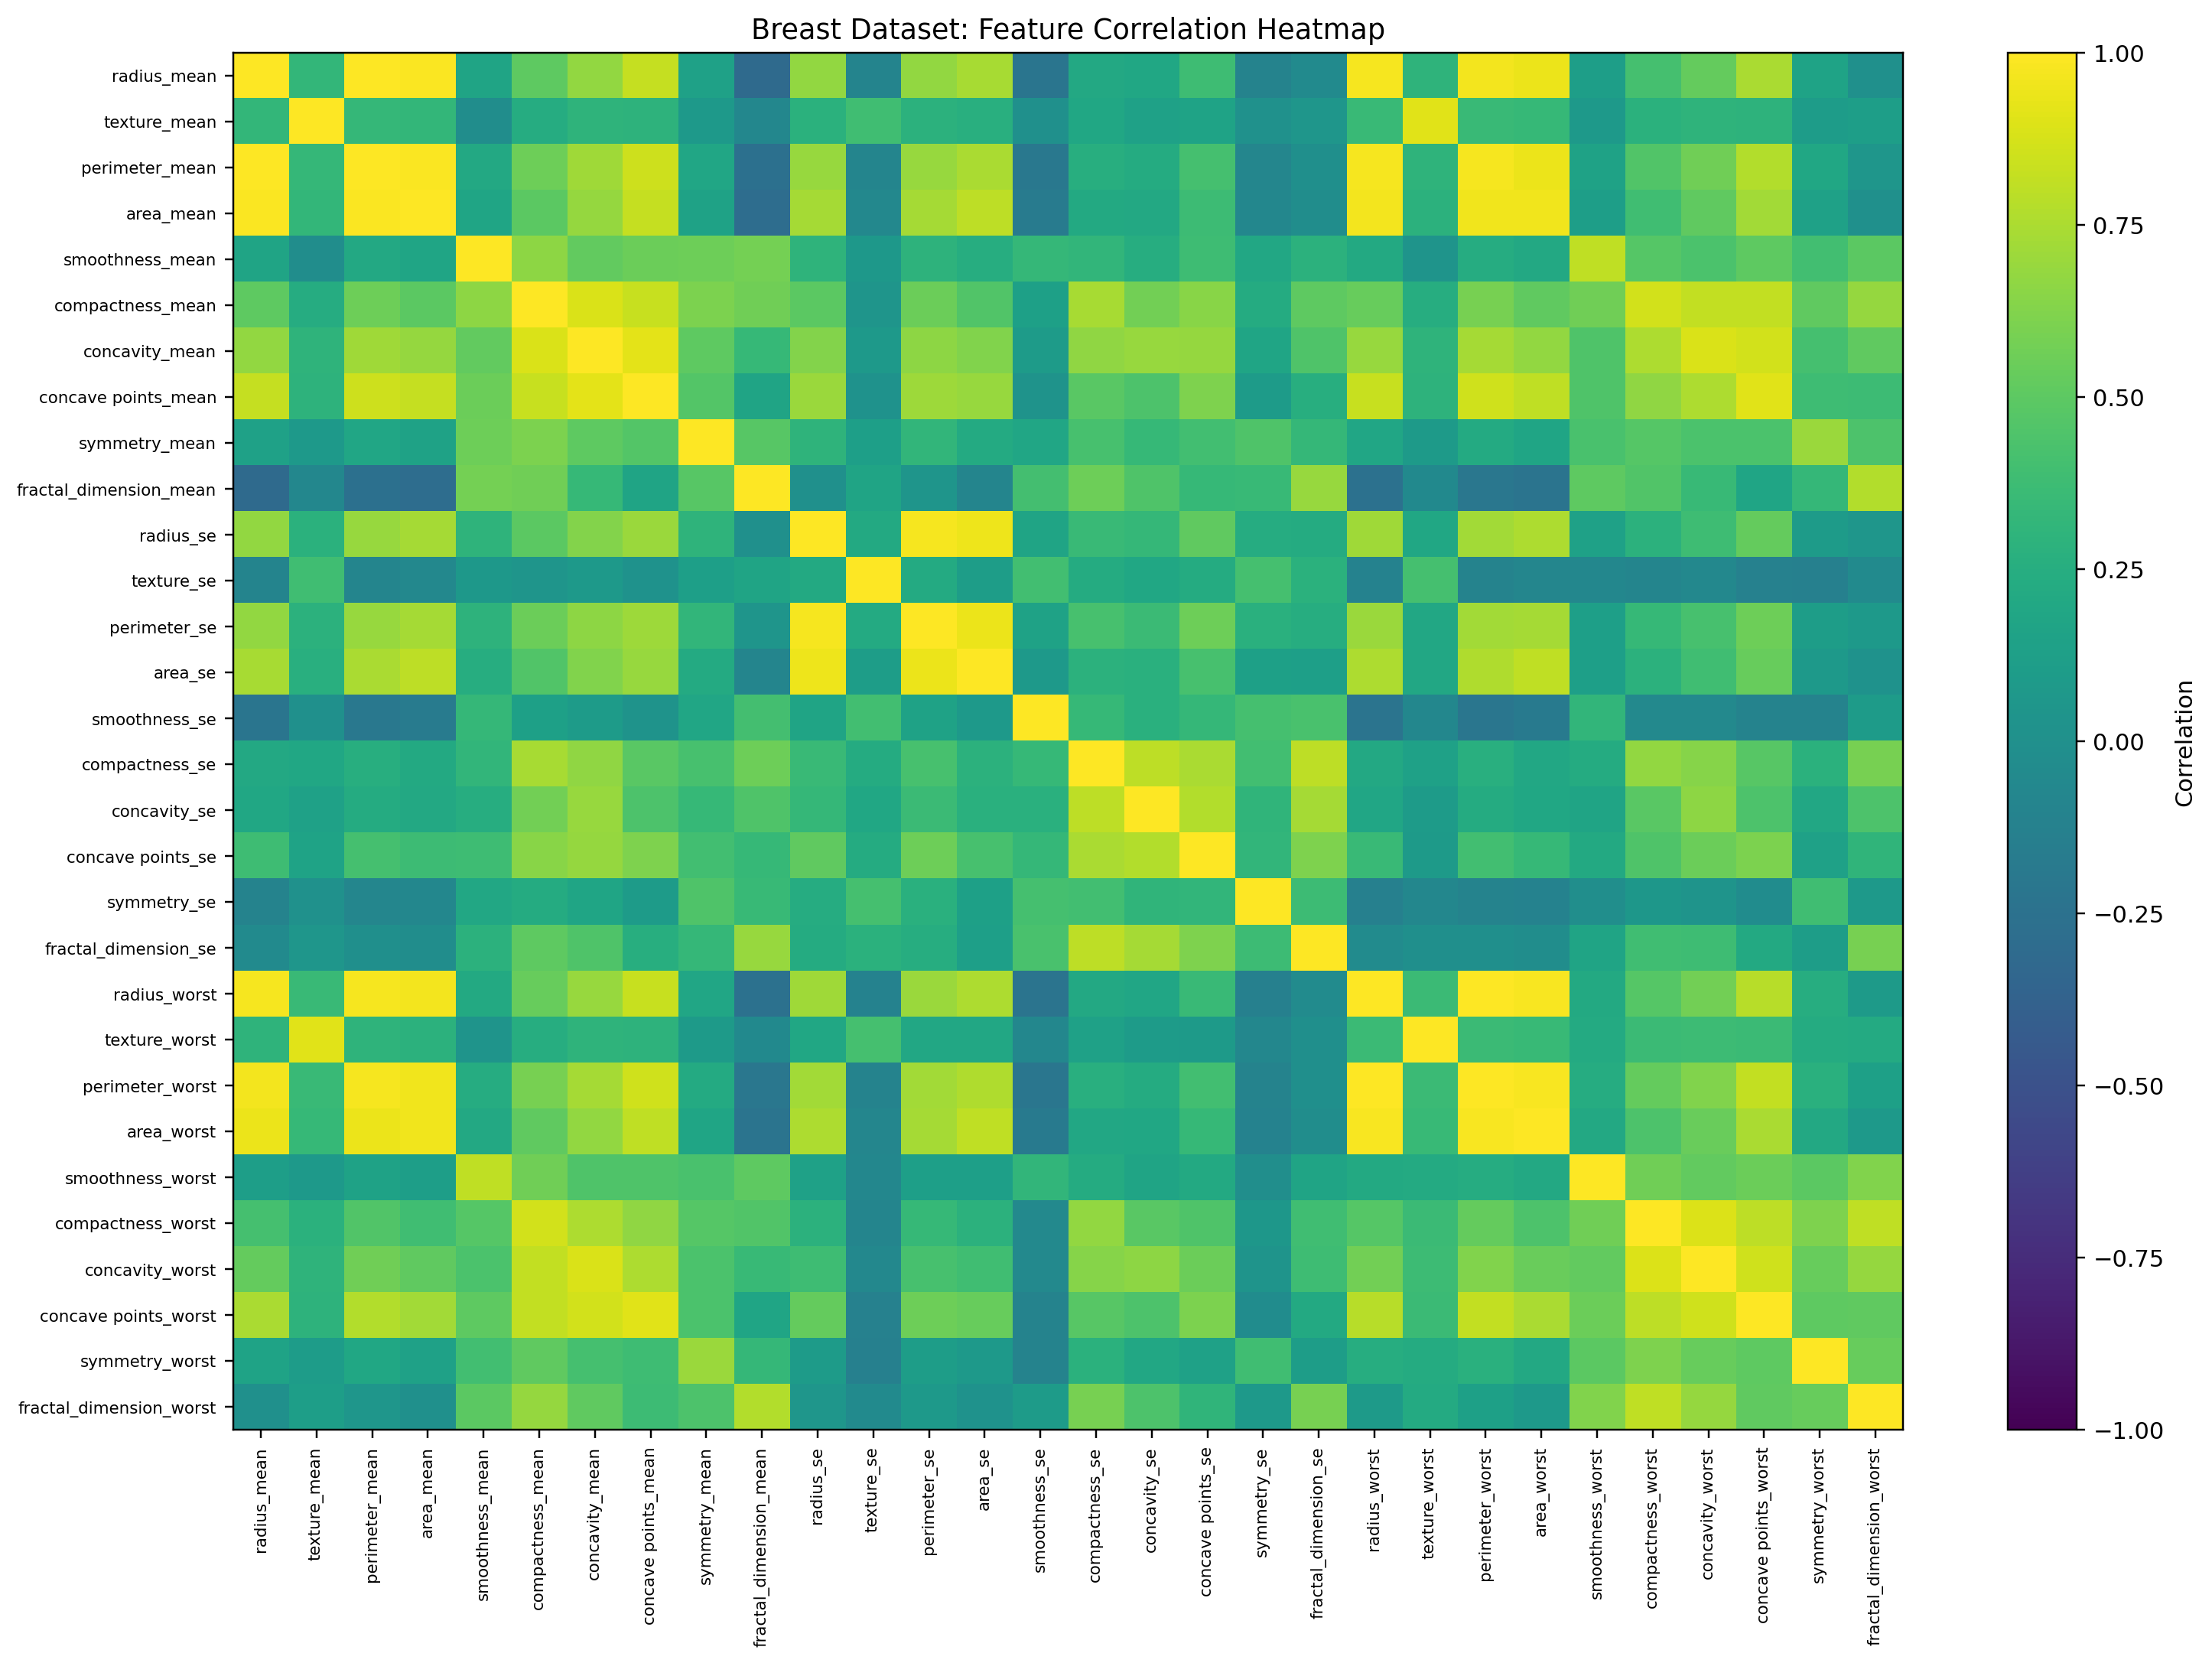
\includegraphics[width=0.47\textwidth]{breast_correlation_heatmap.png}\hfill
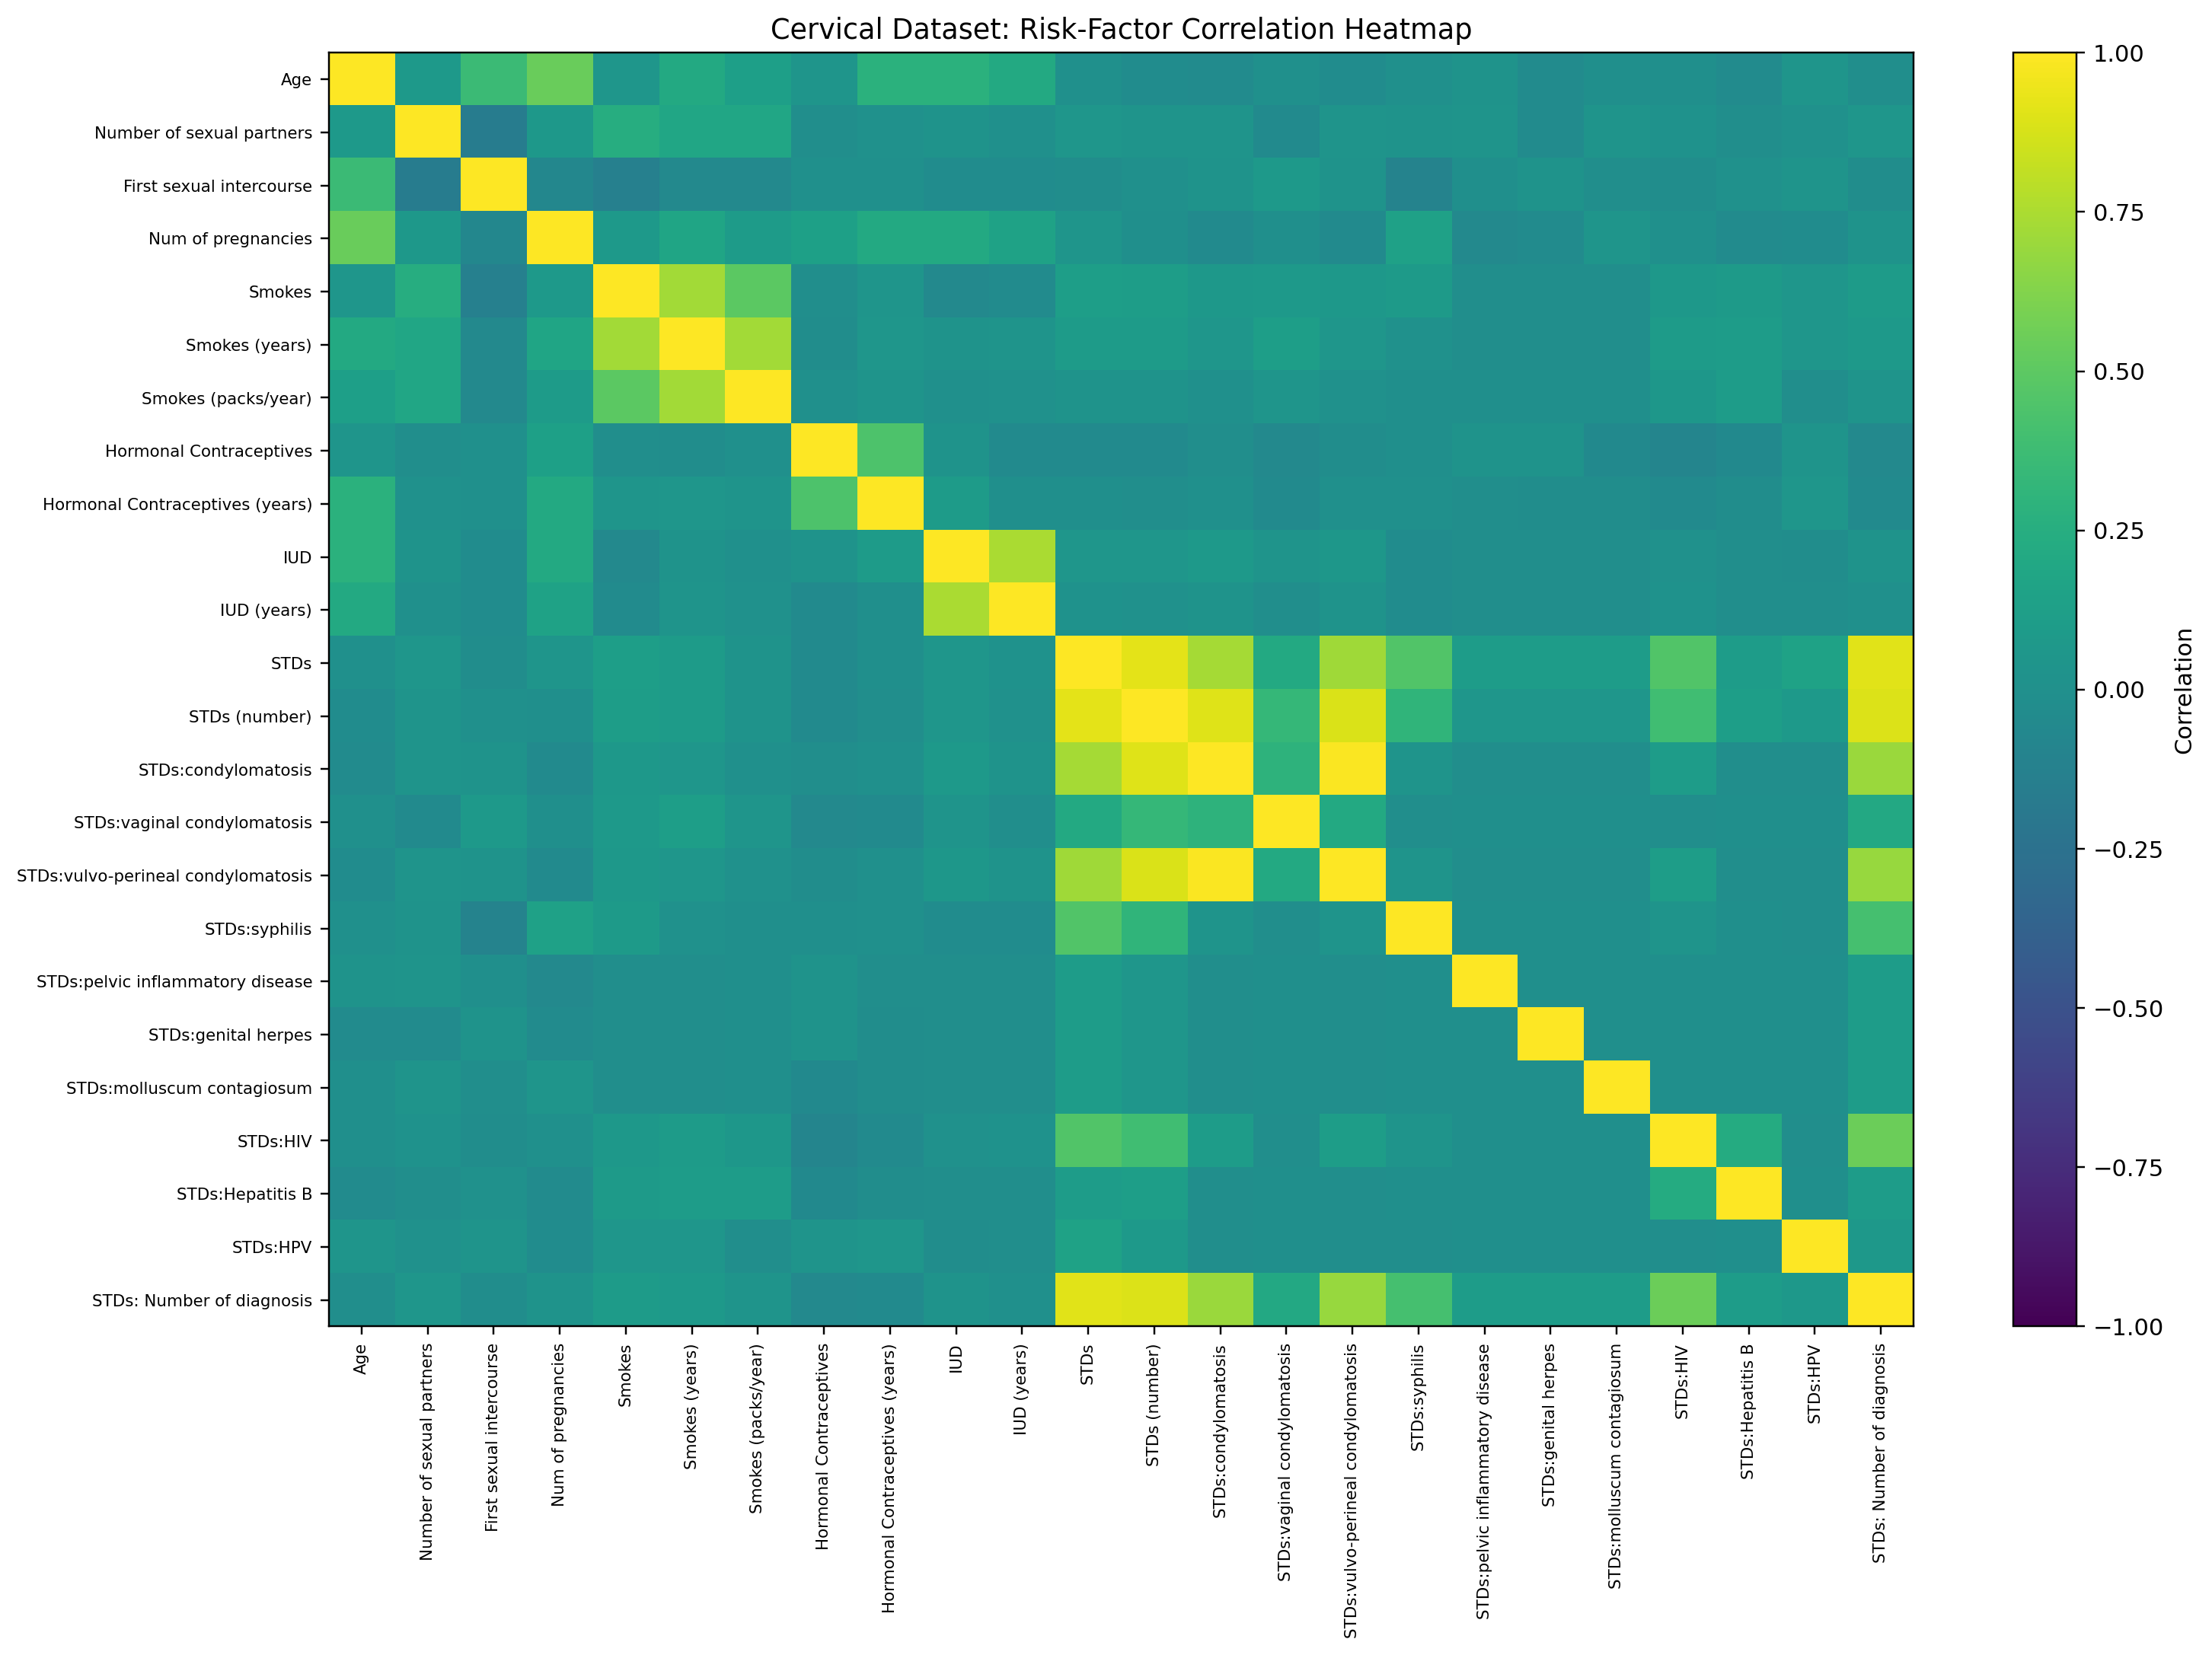
\includegraphics[width=0.47\textwidth]{cervical_correlation_heatmap.png}
\caption{Exploratory feature-correlation heatmaps. Left: breast nuclear measurements. Right: cervical risk-factor/history inputs after exploratory removal of high-missingness and constant columns. These are exploratory associations and do not imply causal relationships.}
\label{fig:correlations}
\end{figure*}

\section{Methodology}
\subsection{Bayes' theorem and class priors}
For classes $C_k$ and an input vector $\mathbf{x}$, Bayes' theorem gives
\begin{equation}
P(C_k\mid\mathbf{x})=\frac{P(C_k)P(\mathbf{x}\mid C_k)}{P(\mathbf{x})}.
\label{eq:bayes}
\end{equation}
The prior probability is estimated from the training data as
\begin{equation}
\widehat{P}(C_k)=\frac{N_k}{N},
\label{eq:prior}
\end{equation}
where $N_k$ is the number of training records in class $C_k$ and $N$ is the total training size. Priors therefore reflect the class proportions in the training partition, not the test set. In the breast experiment the malignant prior is about 0.374; in the cervical experiment the biopsy-positive prior is about 0.064.

\subsection{Gaussian likelihood and maximum-likelihood estimates}
For feature $j$ and class $C_k$, Gaussian Naive Bayes estimates the class-specific mean and population variance by
\begin{align}
\widehat{\mu}_{kj}&=\frac{1}{N_k}\sum_{i:y_i=C_k}x_{ij},\\
\widehat{\sigma}^{2}_{kj}&=\frac{1}{N_k}\sum_{i:y_i=C_k}(x_{ij}-\widehat{\mu}_{kj})^2+\epsilon.
\label{eq:params}
\end{align}
The small additive $\epsilon$ stabilises calculations when a feature variance is extremely small. The implementation uses the variance-smoothing setting $10^{-9}$ multiplied by the largest global feature variance, following the convention of scikit-learn's GaussianNB estimator \cite{sklearnNB}. The resulting smoothing values were $3.383817\times10^{-4}$ for breast and $7.348189\times10^{-8}$ for cervical inputs.

The Gaussian likelihood of one feature value is
\begin{equation}
P(x_j\mid C_k)=\frac{1}{\sqrt{2\pi\widehat{\sigma}^{2}_{kj}}}
\exp\!\left[-\frac{(x_j-\widehat{\mu}_{kj})^2}{2\widehat{\sigma}^{2}_{kj}}\right].
\label{eq:gaussian}
\end{equation}
The numerical value is a probability density, not the probability of one exact continuous value. A larger density means that the observed feature is more compatible with that class's fitted Gaussian distribution.

\subsection{Conditional independence and posterior prediction}
The Naive Bayes assumption states that the features are conditionally independent given the class. Thus,
\begin{equation}
P(\mathbf{x}\mid C_k)\approx\prod_{j=1}^{d}P(x_j\mid C_k),
\label{eq:independence}
\end{equation}
and the predicted class is
\begin{equation}
\widehat{C}=\arg\max_{C_k}\widehat{P}(C_k)
\prod_{j=1}^{d}P(x_j\mid C_k).
\label{eq:decision}
\end{equation}
The implementation sums log-likelihoods rather than multiplying many small density values directly; this reduces numerical underflow. After normalisation, posterior probabilities are returned for both classes. This factorisation also makes the model's assumptions visible: strong feature dependence can lead to over-counting related evidence.

\subsection{Worked probability examples}
For the breast training partition, the median of \texttt{radius\_mean} is 13.34. The observed conditional fraction of malignant records among training cases whose mean radius exceeds this median is
\begin{equation}
P(M\mid\texttt{radius\_mean}>13.34)\approx0.6828.
\end{equation}
This is an empirical conditional probability, not a causal claim. Class-conditional Gaussian estimates for \texttt{radius\_mean} are $\mu_B=12.15549$, $\sigma_B^2=3.16543$ and $\mu_M=17.53676$, $\sigma_M^2=10.76441$ before smoothing. For the illustrative test record with radius mean 11.41, the one-feature Bayes calculation gives posterior probabilities of 94.18\% benign and 5.82\% malignant. This illustration uses only one feature; the full GNB classifier combines all retained features.

For cervical training data, the median age is 26. Among training records above that age, the observed positive biopsy fraction is approximately 6.86\%. For an illustrative test record of age 41, an age-only calculation gives a positive-biopsy posterior of 8.92\%. Age alone is not the full classifier, and this single-feature probability must not be interpreted as an individual's clinical risk.

\begin{figure*}[!t]
\centering
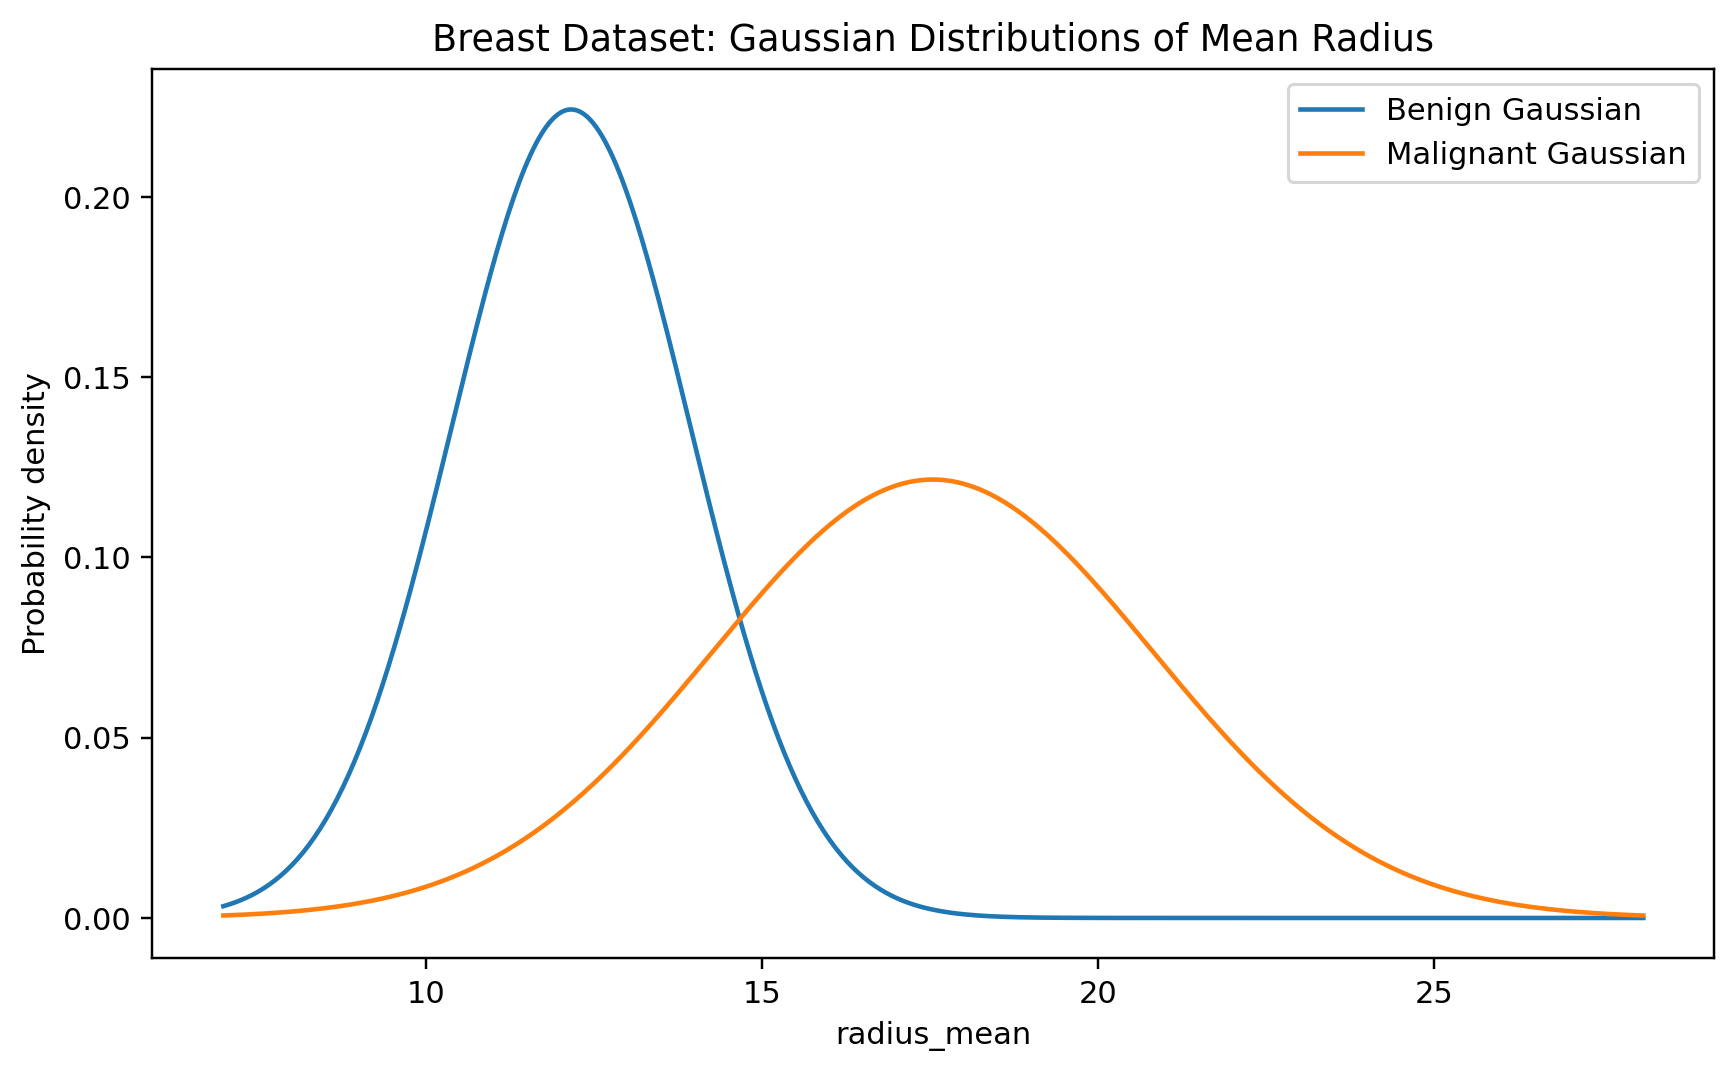
\includegraphics[width=0.47\textwidth]{breast_gaussian_radius_curves.png}\hfill
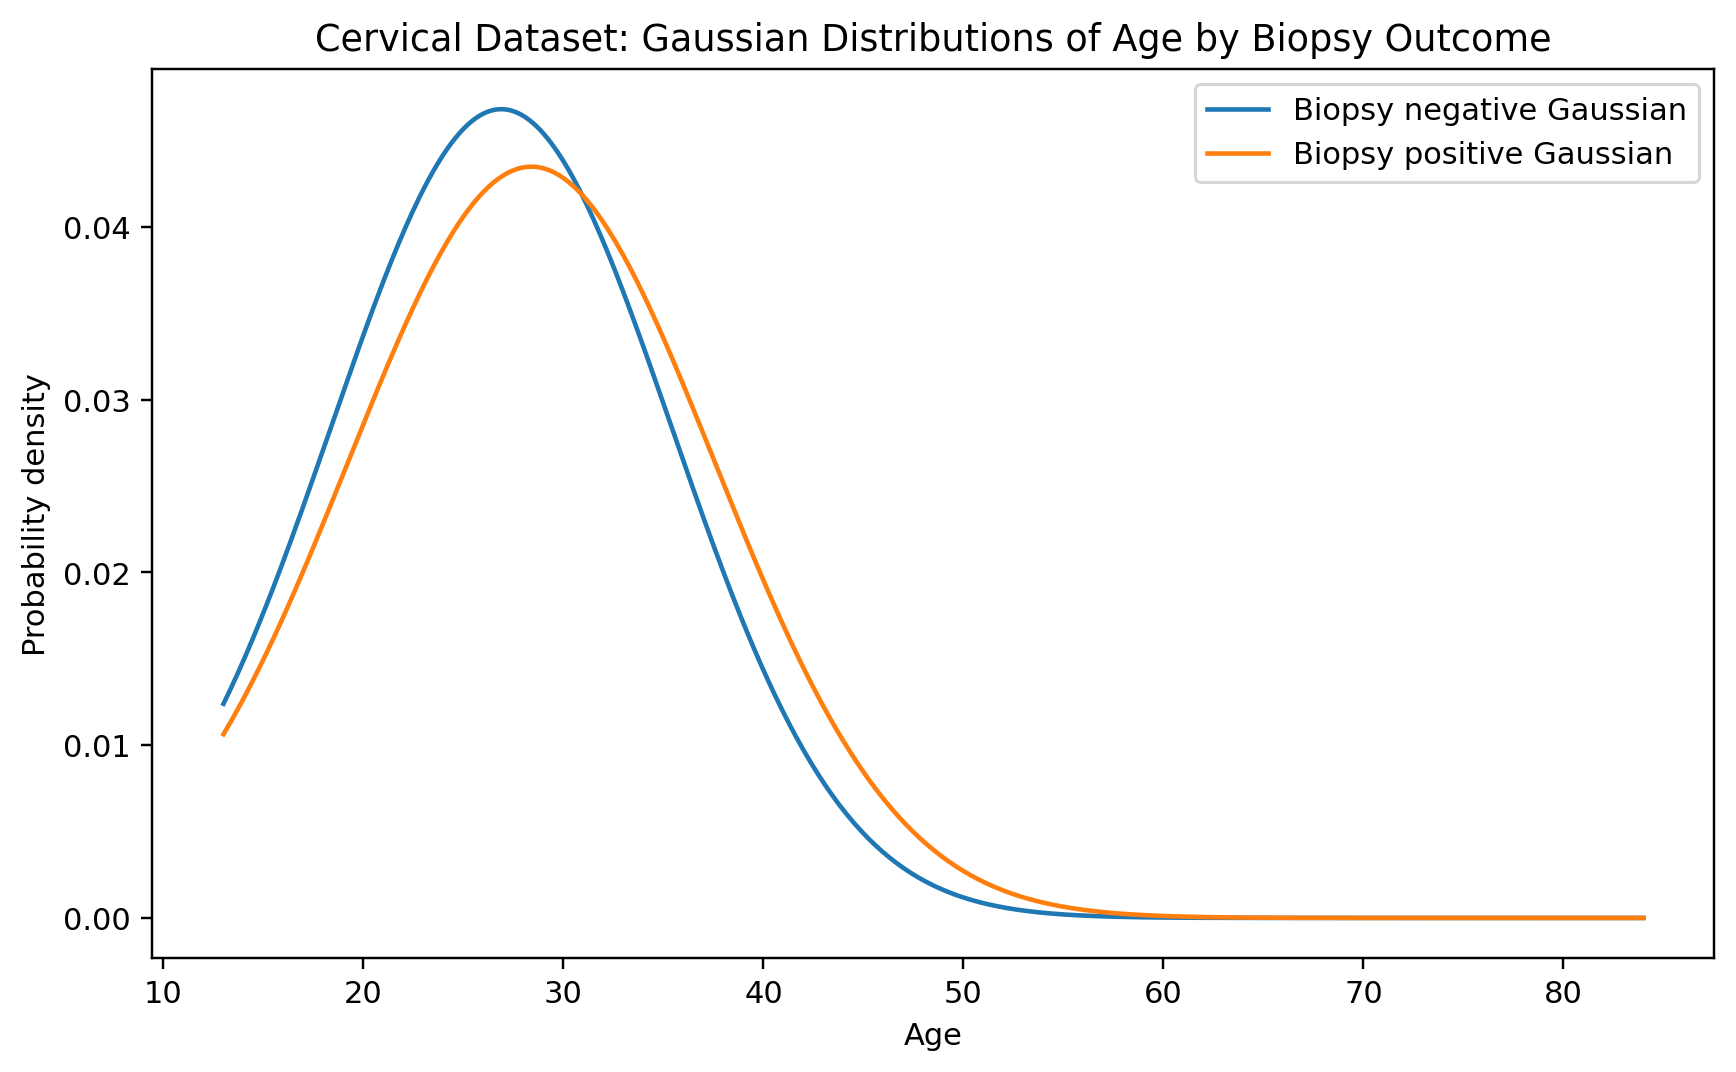
\includegraphics[width=0.47\textwidth]{cervical_gaussian_age_curves.png}
\caption{Illustrative class-conditional Gaussian densities estimated from training data. Left: breast \texttt{radius\_mean} by diagnosis. Right: age by recorded biopsy outcome. The cervical positive-class estimate is based on a small number of observations and should be interpreted cautiously.}
\label{fig:gaussian}
\end{figure*}

\subsection{Models and implementation validation}
Four models and one baseline are compared. (1) Scratch GNB implements class priors, feature-wise means and variances, Gaussian log-likelihoods, posterior normalisation, and maximum-posterior prediction. (2) Scikit-learn GaussianNB uses the same training/test split, median-imputed feature matrix, and smoothing value; the software ecosystem is described by Pedregosa \textit{et al.} \cite{pedregosa}. (3) Logistic Regression uses a median imputer, standardisation, and a Logistic Regression estimator. (4) Balanced Logistic Regression adds \texttt{class\_weight=balanced}. (5) The prior baseline predicts the majority training class, providing a reference for the danger of accuracy under imbalance.

For GNB, missingness and constant-feature decisions are made using training data only; medians are learned only from training data. In Logistic Regression pipelines, imputation and scaling are also fitted within the training data. The experiments use a stratified 80:20 train/test split with \texttt{random\_state=42}. Models use the default 0.5 probability threshold for the binary prediction; no threshold is tuned on the test set.

The scratch model is compared directly against scikit-learn GNB. There are zero differing hard predictions for each dataset. The maximum absolute difference in predicted positive-class probabilities is $7.77\times10^{-16}$ for breast and $1.78\times10^{-15}$ for cervical. These differences are at floating-point precision scale and indicate that the scratch implementation reproduces the library calculation for these experiments. Rounded ROC-AUC values should be used when comparing the two nearly identical implementations.

\subsection{Evaluation metrics}
Let TP, TN, FP, and FN denote true positives, true negatives, false positives, and false negatives. The report uses
\begin{align}
\text{Accuracy}&=\frac{TP+TN}{TP+TN+FP+FN},\\
\text{Precision}&=\frac{TP}{TP+FP},\qquad
\text{Recall}=\frac{TP}{TP+FN},\\
F_1&=2\frac{\text{Precision}\times\text{Recall}}{\text{Precision}+\text{Recall}},\\
\text{Balanced Accuracy}&=\frac{1}{2}\left(\frac{TP}{TP+FN}+\frac{TN}{TN+FP}\right).
\end{align}
ROC-AUC evaluates ranking over classification thresholds, while average precision summarises the precision-recall curve. Precision, recall, F1, balanced accuracy, and average precision are particularly important in the cervical experiment because positive cases are rare \cite{saito}. Metrics are calculated from the held-out test set; cross-validation values are reported separately and use only the training partition.

\section{Experimental Results}
\subsection{Breast diagnostic classification}
On the 114-case breast test set, scratch GNB achieves 93.86\% accuracy, 91.67\% balanced accuracy, 100\% precision, 83.33\% recall, and 0.909 F1 for the malignant class. It predicts no benign case as malignant (zero false positives), but misses seven of the 42 malignant cases. Its ROC-AUC is 0.993 and average precision is 0.989, indicating strong score separation on this split despite the seven missed malignant cases.

Logistic Regression improves the test recall to 92.86\% and F1 to 0.951. Balanced Logistic Regression obtains 97.37\% accuracy, 96.92\% balanced accuracy, 95.24\% recall, and 0.964 F1. It makes two false-negative predictions and one false-positive prediction. Thus, among the tested models, balanced Logistic Regression offers the strongest threshold-based test results for this particular split; standard GNB remains the project's primary probabilistic model because it directly demonstrates the prescribed probability and density-estimation concepts.

\begin{table*}[!t]
\centering
\caption{Breast Test-Set Metrics (Malignant Is the Positive Class)}
\label{tab:breastmetrics}
\scriptsize
\setlength{\tabcolsep}{5pt}
\begin{tabular}{lrrrrrrr}
\toprule
Model & Accuracy & Bal. Acc. & Precision & Recall & $F_1$ & ROC-AUC & Avg. Prec. \\
\midrule
Scratch GNB & 0.939 & 0.917 & 1.000 & 0.833 & 0.909 & 0.993 & 0.989 \\
Scikit-learn GNB & 0.939 & 0.917 & 1.000 & 0.833 & 0.909 & 0.993 & 0.989 \\
Logistic Regression & 0.965 & 0.957 & 0.975 & 0.929 & 0.951 & 0.996 & 0.994 \\
Balanced Logistic Regression & 0.974 & 0.969 & 0.976 & 0.952 & 0.964 & 0.995 & 0.993 \\
Prior baseline & 0.632 & 0.500 & 0.000 & 0.000 & 0.000 & 0.500 & 0.368 \\
\bottomrule
\end{tabular}
\end{table*}

\subsection{Cervical biopsy-outcome classification}
The cervical test set contains 156 negative and only 11 positive biopsy records. Scratch GNB achieves 10.78\% accuracy, 48.02\% balanced accuracy, 6.33\% precision, 90.91\% recall, 0.118 F1, 0.642 ROC-AUC, and 0.133 average precision. It correctly flags 10 of the 11 positive records, but predicts positive for 158 test records, of which 148 are false positives. The low precision and high false-positive count mean that the high recall does not translate into useful classification at the default threshold.

Standard Logistic Regression has 92.81\% accuracy but predicts none of the 11 positive cases correctly. Its positive-class recall and F1 are zero. The majority-class prior baseline is similarly misleading: it reaches 93.41\% accuracy by predicting every test record as negative, while missing all positive biopsy outcomes. Balanced Logistic Regression improves positive-class recall to 36.36\% and F1 to 0.190, with a balanced accuracy of 59.53\%; it detects four of the 11 positive test cases and yields 27 false positives. Its ROC-AUC (0.662) is the highest in this cervical test comparison, but the absolute discrimination remains modest and the test set is small.

\begin{table*}[!t]
\centering
\caption{Cervical Test-Set Metrics (Biopsy-Positive Is the Positive Class)}
\label{tab:cervicalmetrics}
\scriptsize
\setlength{\tabcolsep}{5pt}
\begin{tabular}{lrrrrrrr}
\toprule
Model & Accuracy & Bal. Acc. & Precision & Recall & $F_1$ & ROC-AUC & Avg. Prec. \\
\midrule
Scratch GNB & 0.108 & 0.480 & 0.063 & 0.909 & 0.118 & 0.642 & 0.133 \\
Scikit-learn GNB & 0.108 & 0.480 & 0.063 & 0.909 & 0.118 & 0.642 & 0.129 \\
Logistic Regression & 0.928 & 0.497 & 0.000 & 0.000 & 0.000 & 0.640 & 0.113 \\
Balanced Logistic Regression & 0.796 & 0.595 & 0.129 & 0.364 & 0.190 & 0.662 & 0.105 \\
Prior baseline & 0.934 & 0.500 & 0.000 & 0.000 & 0.000 & 0.500 & 0.066 \\
\bottomrule
\end{tabular}
\end{table*}

\begin{figure*}[!t]
\centering
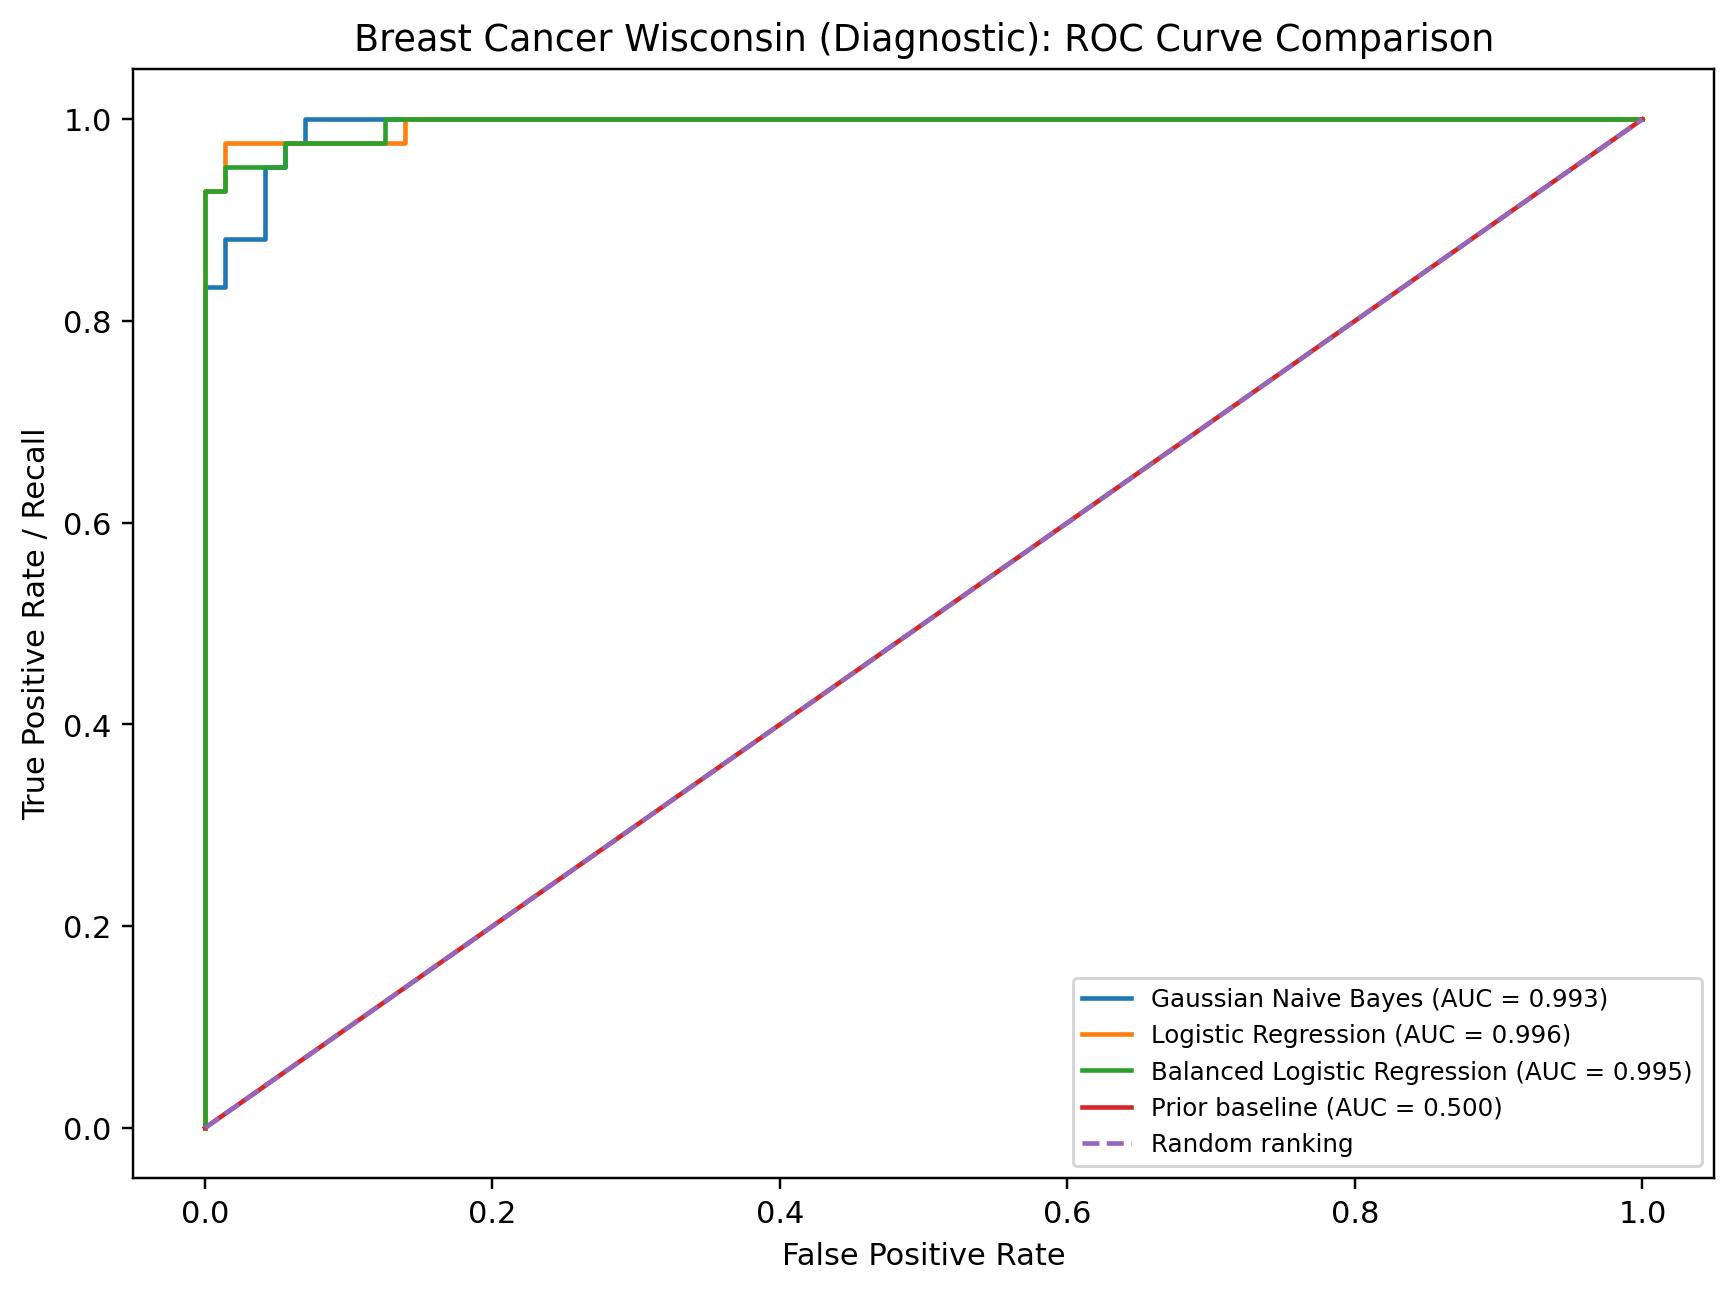
\includegraphics[width=0.47\textwidth]{breast_roc_curves.png}\hfill
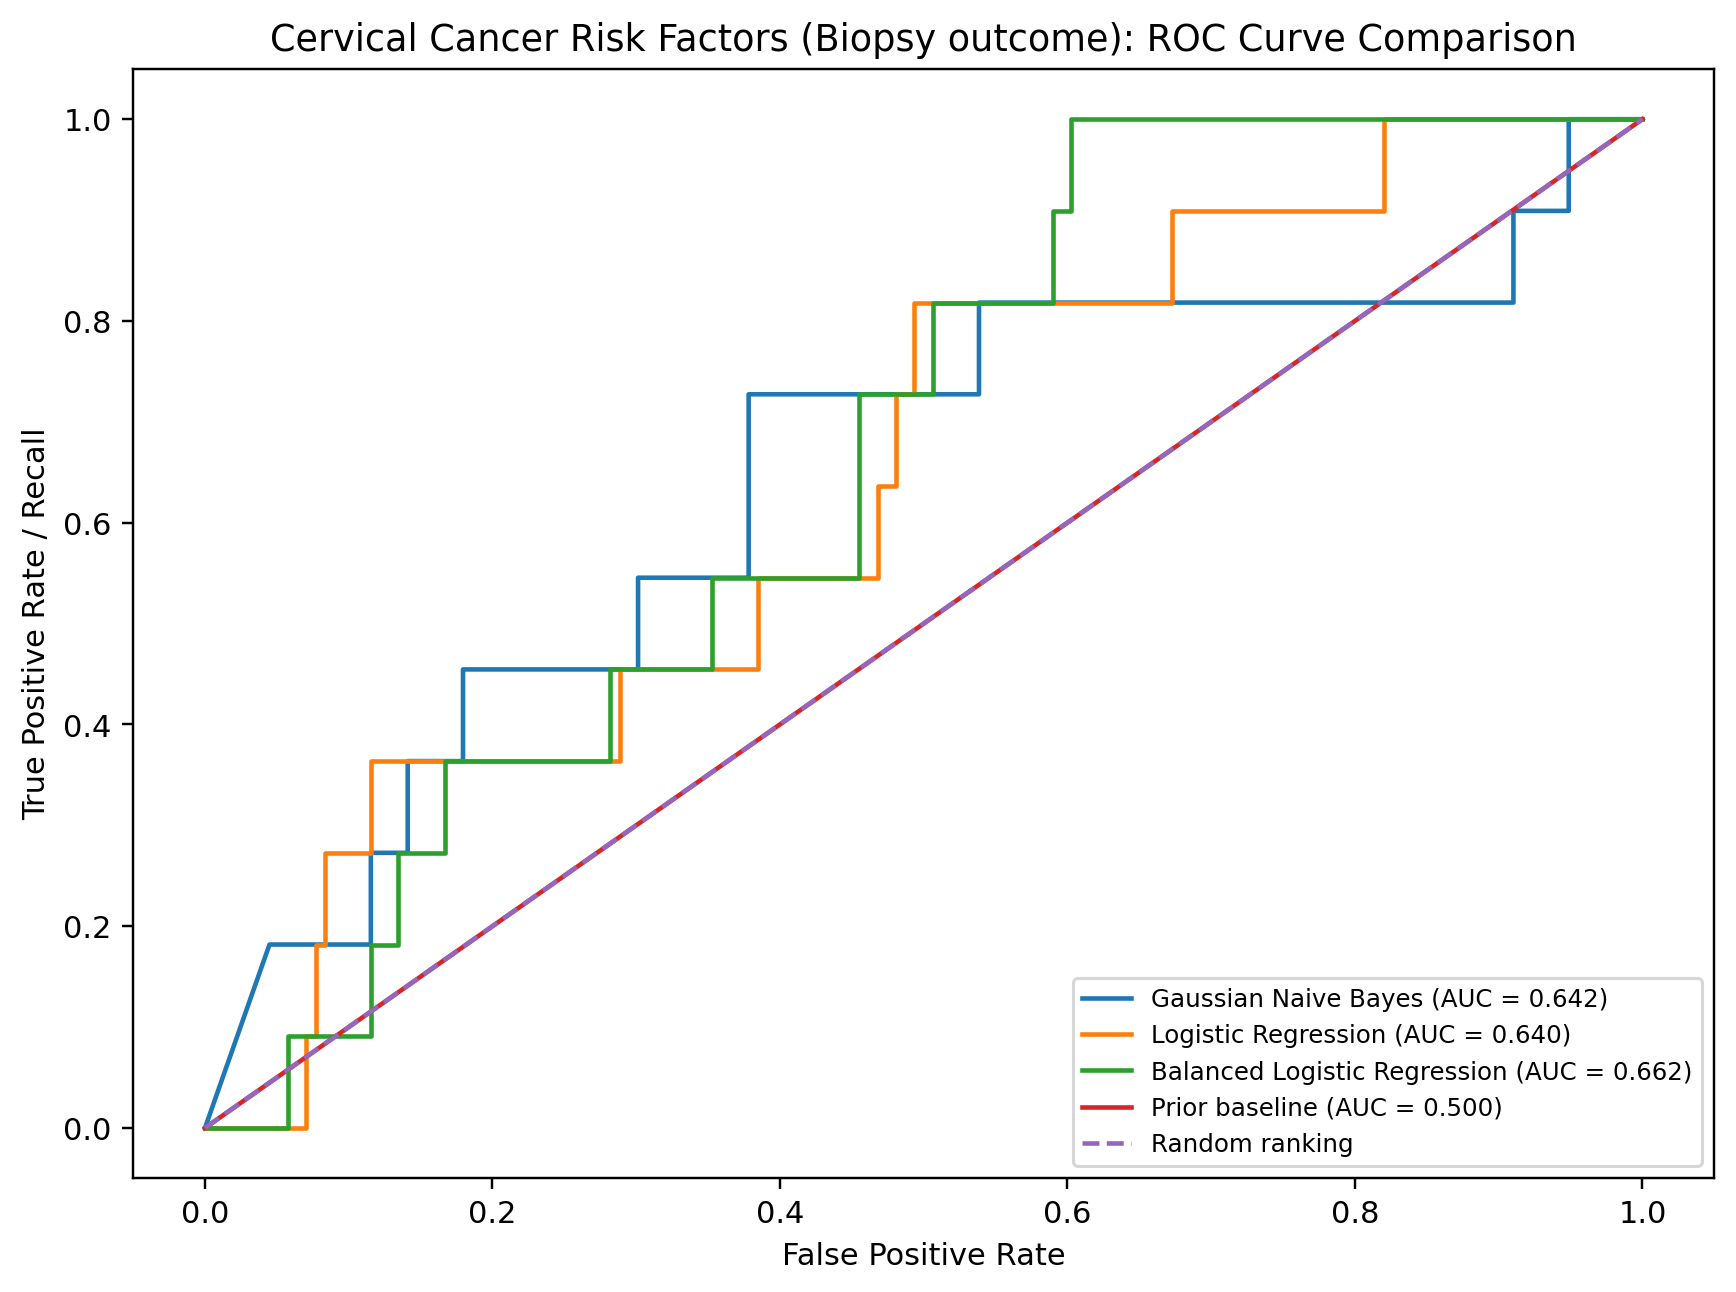
\includegraphics[width=0.47\textwidth]{cervical_roc_curves.png}
\caption{ROC curves for the two independent test experiments. Left: strong ranking performance on the breast dataset. Right: modest discrimination on the cervical biopsy-outcome task. ROC-AUC does not by itself select a useful operating threshold, and it must be interpreted with the precision-recall results and confusion matrices.}
\label{fig:roc}
\end{figure*}

\subsection{Five-fold cross-validation on training partitions}
As a robustness check, stratified five-fold cross-validation with shuffling and a fixed seed is run on the training partition only. Each fold fits its own imputation and scaling steps. The table entries show mean and sample standard deviation across the five held-out folds. Scratch GNB is not included in cross-validation; the library GNB implementation is used for that part of the comparison.

For the breast dataset, cross-validated Logistic Regression has mean accuracy 0.974, balanced accuracy 0.969, recall 0.953, F1 0.964, ROC-AUC 0.996, and average precision 0.995. Balanced Logistic Regression has similar scores, with mean recall 0.959 and F1 0.962. Library GNB gives mean accuracy 0.941 and ROC-AUC 0.988. These results support the test-split finding that the linear models perform at least as well as GNB on this dataset, although fold averages are not guarantees of future performance.

For the cervical task, the mean accuracy of the prior baseline is 0.936 but its mean recall and F1 are both zero. GNB's cross-validated mean recall is 1.000, paired with mean accuracy 0.106, balanced accuracy 0.522, precision 0.067, and F1 0.126. This again indicates extensive positive predictions and many false positives. Balanced Logistic Regression increases the mean balanced accuracy to 0.604 and mean recall to 0.419, but its F1 remains low (0.183) and the standard deviations are sizeable relative to the means. The scarcity of positive cases in each validation fold limits the precision of these estimates.

\begin{table*}[!t]
\centering
\caption{Five-Fold Cross-Validation on the Breast Training Partition: Mean $\pm$ Standard Deviation}
\label{tab:breastcv}
\scriptsize
\setlength{\tabcolsep}{4pt}
\begin{tabular}{lrrrrrr}
\toprule
Model & Accuracy & Bal. Acc. & Recall & $F_1$ & ROC-AUC & Avg. Prec. \\
\midrule
Scikit-learn GNB & $0.941\pm0.030$ & $0.932\pm0.034$ & $0.900\pm0.061$ & $0.919\pm0.040$ & $0.988\pm0.008$ & $0.982\pm0.013$ \\
Logistic Regression & $0.974\pm0.017$ & $0.969\pm0.021$ & $0.953\pm0.045$ & $0.964\pm0.023$ & $0.996\pm0.005$ & $0.995\pm0.005$ \\
Balanced Logistic Regression & $0.971\pm0.020$ & $0.969\pm0.022$ & $0.959\pm0.034$ & $0.962\pm0.027$ & $0.995\pm0.005$ & $0.994\pm0.005$ \\
Prior baseline & $0.626\pm0.000$ & $0.500\pm0.000$ & $0.000\pm0.000$ & $0.000\pm0.000$ & $0.500\pm0.000$ & $0.374\pm0.000$ \\
\bottomrule
\end{tabular}
\end{table*}

\begin{table*}[!t]
\centering
\caption{Five-Fold Cross-Validation on the Cervical Training Partition: Mean $\pm$ Standard Deviation}
\label{tab:cervicalcv}
\scriptsize
\setlength{\tabcolsep}{4pt}
\begin{tabular}{lrrrrrr}
\toprule
Model & Accuracy & Bal. Acc. & Recall & $F_1$ & ROC-AUC & Avg. Prec. \\
\midrule
Scikit-learn GNB & $0.106\pm0.010$ & $0.522\pm0.005$ & $1.000\pm0.000$ & $0.126\pm0.007$ & $0.609\pm0.133$ & $0.158\pm0.071$ \\
Logistic Regression & $0.931\pm0.003$ & $0.509\pm0.025$ & $0.025\pm0.056$ & $0.036\pm0.081$ & $0.581\pm0.120$ & $0.144\pm0.069$ \\
Balanced Logistic Regression & $0.765\pm0.017$ & $0.604\pm0.084$ & $0.419\pm0.180$ & $0.183\pm0.066$ & $0.581\pm0.132$ & $0.147\pm0.085$ \\
Prior baseline & $0.936\pm0.004$ & $0.500\pm0.000$ & $0.000\pm0.000$ & $0.000\pm0.000$ & $0.500\pm0.000$ & $0.064\pm0.004$ \\
\bottomrule
\end{tabular}
\end{table*}

\section{Discussion}
\subsection{What the breast experiment shows}
The breast results demonstrate that class priors and Gaussian feature likelihoods can combine into effective posterior ranking for this dataset. Scratch GNB and the standard implementation agree numerically, and the resulting test ROC-AUC is high. Nonetheless, GNB's default-threshold confusion matrix contains seven false negatives. In a task where failing to flag a malignant record may be important, recall and the consequences of the errors must be considered alongside overall accuracy. Logistic Regression and balanced Logistic Regression detect more malignant cases on this particular split while introducing a small number of false positives. A high ROC-AUC describes score ranking across thresholds; it is not proof that a chosen threshold is clinically appropriate.

The observed differences among models should not be interpreted as a universal ranking. They depend on this dataset, the selected split, the definitions of positive class, preprocessing, and the operating threshold. The breast dataset is a well-structured benchmark with 569 observations, but the strong correlations among morphometric features make the GNB independence assumption questionable. That limitation helps explain why a model with simpler independent likelihoods may be outperformed by Logistic Regression while remaining useful as a teaching model.

\subsection{Why cervical accuracy is misleading}
The cervical experiment illustrates a more severe class-imbalance problem. A classifier predicting every record as biopsy-negative receives about 93.4\% accuracy because negative outcomes dominate the test set, yet its positive-class recall is zero. Conversely, GNB catches most positive test cases but labels nearly the entire negative class as positive. The false-positive count (148) reduces precision to 6.33\%. Neither behaviour should be described as good classification merely because one headline metric looks high.

Balanced Logistic Regression provides a more moderate trade-off, with four true positives, seven false negatives, and 27 false positives on the test split. It achieves the highest cervical ROC-AUC among the four trained/baseline comparisons (0.662), but the result remains modest, its F1-score is only 0.190, and only 11 positive cases are in the test set. A small change in the classification of one positive record changes recall by about 9.1 percentage points. The cross-validation standard deviations similarly show substantial variability. Further methodological work could examine threshold selection using validation-only data, better treatment of mixed binary/continuous variables, carefully justified resampling or cost-sensitive learning, calibrated probabilities, and external evaluation. Such options are future work, not evidence that the current model is ready for screening.

\subsection{Interpretation of model agreement}
The from-scratch implementation is validated by matching the standard GaussianNB implementation using the same preprocessing and feature matrix. The zero hard-label disagreements and probability differences near machine precision provide evidence that the implementation is internally consistent with the reference software. This validates the code path; it does not validate the assumptions of Gaussian Naive Bayes, establish the correctness of the dataset labels, or prove clinical usefulness. In particular, an algorithm can be implemented correctly and still yield poor predictions for an imbalanced task.

\subsection{Threats to validity}
First, both experiments use a single random held-out split from the same source datasets, with cross-validation limited to the training partition. There is no independent external test population. Second, the cervical dataset has only 54 biopsy-positive records before splitting and 11 in the test set; precision and recall estimates are therefore uncertain. Third, GNB treats every feature as Gaussian and conditionally independent within each class. This is a rough approximation for binary or discrete cervical variables and correlated breast measurements. Fourth, median imputation may be convenient but can obscure informative missingness and does not solve sampling bias. Fifth, the chosen class threshold is the default 0.5 probability threshold; the report does not tune it against a clinical utility function. Finally, biopsy outcome is the recorded target in the cervical experiment, and should not be conflated with a full cancer diagnosis or population screening outcome.

\section{Conclusion and Future Work}
This project demonstrates how conditional probability, Gaussian distributions, maximum-likelihood parameter estimation, likelihoods, and Bayes' theorem can be translated into an interpretable classification algorithm. On the Breast Cancer Wisconsin (Diagnostic) test split, scratch GNB obtains 93.86\% accuracy and 0.993 ROC-AUC, while balanced Logistic Regression performs best among the tested models for several threshold-based metrics. The scratch GNB predictions match scikit-learn's predictions for both datasets, validating the implementation. The cervical biopsy-outcome experiment is much more difficult: class imbalance creates a large separation between accuracy, recall, precision, and F1, and none of the tested models produces strong performance across all metrics.

The key statistical lesson is that priors, likelihood assumptions, and class imbalance shape a classifier's predictions. Accuracy alone can be inadequate, and model implementation correctness does not imply domain validity. Future work should test decision thresholds on a validation set, compare models suitable for mixed data types, investigate calibration and missingness, and evaluate using an independent dataset with a carefully defined target. These results are intended for coursework and should not be used to diagnose cancer or determine treatment for any person.

\section*{Reproducibility and Code}
The experiments were implemented in Python using NumPy, pandas, Matplotlib, and scikit-learn. The notebook uses a stratified train/test split (test size 0.20, random state 42) and a stratified five-fold cross-validation procedure on the training data. The notebook, prediction tables, metric summaries, validation checks, and figures are included with the report source bundle. To reproduce the results, place the two CSV files at the paths specified in the notebook, install the listed Python dependencies, and run all cells from top to bottom. Because the notebook writes plots and CSV outputs, the output folder must be writable. Exact package versions may affect last-decimal rounding.

\section*{Acknowledgment}
This work was prepared as a Probability and Statistics (BAMAT207) course project under Track 6: AI, Machine Learning and Probability.

\appendices
\section{Held-Out Confusion-Matrix Counts}
Table~\ref{tab:confusions} provides the exact test-set counts underlying the threshold-based metrics. Rows are the actual class and columns are predicted classes: TN and TP are correct decisions, while FP and FN are errors. These counts illustrate why models must be evaluated against the task rather than accuracy alone. In the cervical task, the GNB model labels 148 of 156 biopsy-negative records as positive, while the prior baseline labels every record negative and misses all 11 positive cases.

\begin{center}
\refstepcounter{table}\label{tab:confusions}
{\footnotesize TABLE \thetable\par}
{\footnotesize\textsc{Confusion-Matrix Counts for the Held-Out Test Sets}\par}
\vspace{2pt}
\scriptsize
\setlength{\tabcolsep}{3pt}
\begin{tabular}{p{1.05cm}p{2.05cm}rrrr}
\toprule
Task & Model & TN & FP & FN & TP \\
\midrule
Breast & Scratch GNB & 72 & 0 & 7 & 35 \\
Breast & Library GNB & 72 & 0 & 7 & 35 \\
Breast & Logistic Reg. & 71 & 1 & 3 & 39 \\
Breast & Balanced Logit. & 71 & 1 & 2 & 40 \\
Breast & Prior baseline & 72 & 0 & 42 & 0 \\
Cervical & Scratch GNB & 8 & 148 & 1 & 10 \\
Cervical & Library GNB & 8 & 148 & 1 & 10 \\
Cervical & Logistic Reg. & 155 & 1 & 11 & 0 \\
Cervical & Balanced Logit. & 129 & 27 & 7 & 4 \\
Cervical & Prior baseline & 156 & 0 & 11 & 0 \\
\bottomrule
\end{tabular}
\end{center}

\section{Implementation Validation and Probability Examples}
The maximum absolute positive-class probability difference between scratch GNB and scikit-learn GNB was $7.77\times10^{-16}$ for breast and $1.78\times10^{-15}$ for cervical. The hard predictions agreed for all 114 breast and all 167 cervical test records. The difference is at floating-point precision scale and supports implementation consistency, not clinical validity.

The single-feature breast example uses $x=11.41$ for \texttt{radius\_mean}. The fitted Gaussian densities are approximately $f(x\mid B)=0.205385$ and $f(x\mid M)=0.021266$; after multiplying by training priors and normalising, $P(B\mid x)=0.941831$ and $P(M\mid x)=0.058169$. In the cervical age example with $x=41$, the respective densities are approximately 0.011887 and 0.016920 for biopsy-negative and biopsy-positive classes. After applying the training priors, the age-only posterior for biopsy-positive is 0.089195. These examples show the mechanics of likelihood and posterior calculation; they are not complete model predictions or medical risk estimates.

\begin{thebibliography}{00}
\bibitem{uciBreast}
W. Wolberg, O. Mangasarian, and N. Street, ``Breast Cancer Wisconsin (Diagnostic),'' UCI Machine Learning Repository, 1993, doi: 10.24432/C5DW2B. [Online]. Available: \url{https://archive.ics.uci.edu/dataset/17/breast-cancer-wisconsin-diagnostic}

\bibitem{street}
W. N. Street, W. H. Wolberg, and O. L. Mangasarian, ``Nuclear feature extraction for breast tumor diagnosis,'' in \emph{Proc. SPIE: Biomedical Image Processing and Biomedical Visualization}, vol. 1905, 1993, pp. 861--870, doi: 10.1117/12.148698.

\bibitem{uciCervical}
K. Fernandes, J. S. Cardoso, and J. Fernandes, ``Cervical Cancer (Risk Factors),'' UCI Machine Learning Repository, 2017, doi: 10.24432/C5Z310. [Online]. Available: \url{https://archive.ics.uci.edu/dataset/383/cervical-cancer}

\bibitem{fernandes}
K. Fernandes, J. S. Cardoso, and J. Fernandes, ``Transfer learning with partial observability applied to cervical cancer screening,'' in \emph{Pattern Recognition and Image Analysis (IbPRIA 2017)}, Lecture Notes in Computer Science, vol. 10255. Cham, Switzerland: Springer, 2017, pp. 243--250, doi: 10.1007/978-3-319-58838-4\_27.

\bibitem{bishop}
C. M. Bishop, \emph{Pattern Recognition and Machine Learning}. New York, NY, USA: Springer, 2006.

\bibitem{sklearnNB}
Scikit-learn Developers, ``Naive Bayes'' and ``GaussianNB,'' scikit-learn documentation. [Online]. Available: \url{https://scikit-learn.org/stable/modules/naive_bayes.html} and \url{https://scikit-learn.org/stable/modules/generated/sklearn.naive_bayes.GaussianNB.html}. Accessed: Oct. 22, 2026.

\bibitem{pedregosa}
F. Pedregosa \textit{et al.}, ``Scikit-learn: Machine learning in Python,'' \emph{Journal of Machine Learning Research}, vol. 12, pp. 2825--2830, 2011.

\bibitem{saito}
T. Saito and M. Rehmsmeier, ``The precision-recall plot is more informative than the ROC plot when evaluating binary classifiers on imbalanced datasets,'' \emph{PLoS ONE}, vol. 10, no. 3, Art. no. e0118432, 2015, doi: 10.1371/journal.pone.0118432.
\end{thebibliography}

\end{document}
